% \documentclass{article}
% \usepackage[dvipsnames]{xcolor}
% \usepackage{tikz}
% \usepackage{xcolor,colortbl}
% 
% \begin{document}
% 
% % - rules etc --------------------------------------------------------------------
\newcommand{\naf}[1]{\ensuremath{{\sim}{#1}}}
\newcommand{\poslits}[1]{\ensuremath{#1^+}}
\newcommand{\neglits}[1]{\ensuremath{#1^-}}
\newcommand{\body}[1]{\ensuremath{B(#1)}} % {\ensuremath{\mathit{body}(#1)}}
\newcommand{\pbody}[1]{\poslits{\body{#1}}} % {\ensuremath{\mathit{body}^+(#1)}}
\newcommand{\nbody}[1]{\neglits{\body{#1}}} % {\ensuremath{\mathit{body}^-(#1)}}
\newcommand{\head}[1]{\ensuremath{h(#1)}} % {\ensuremath{\mathit{head}(#1)}}

\newcommand{\Tsign}{\ensuremath{\mathbf{T}}}
\newcommand{\Fsign}{\ensuremath{\mathbf{F}}}
\newcommand{\Tlit}[1]{\ensuremath{\Tsign #1}}
\newcommand{\Flit}[1]{\ensuremath{\Fsign #1}}
\newcommand{\Ass}{\ensuremath{\mathbf{A}}}
\newcommand{\DL}{\ensuremath{\mathit{DL}}}

\newcommand{\code}[1]{{\ttfamily #1}}
\newcommand{\codeClass}[2]{\code{#2}}

% - systems ----------------------------------------------------------------------
%
\newcommand{\sysfont}{\textit}
\newcommand{\acthex}{\sysfont{acthex}}
\newcommand{\asparagus}{\sysfont{asparagus}}
\newcommand{\aspic}{\sysfont{aspic}}
\newcommand{\aspmt}{\sysfont{aspmt}}
\newcommand{\asprin}{\sysfont{asprin}}
\newcommand{\assat}{\sysfont{assat}}
\newcommand{\berkmin}{\sysfont{berkmin}}
\newcommand{\claspD}{\sysfont{claspD}}
\newcommand{\claspar}{\sysfont{claspar}}
\newcommand{\claspfolio}{\sysfont{claspfolio}}
\newcommand{\clasp}{\sysfont{clasp}}
\newcommand{\clingcon}{\sysfont{clingcon}}
\newcommand{\clingo}{\sysfont{clingo}}
\newcommand{\cmodels}{\sysfont{cmodels}}
\newcommand{\coala}{\sysfont{coala}}
\newcommand{\dingo}{\sysfont{dingo}}
\newcommand{\dflat}{\sysfont{dflat}}
\newcommand{\dlvhex}{\sysfont{dlvhex}}
\newcommand{\dlv}{\sysfont{dlv}}
\newcommand{\ezcsp}{\sysfont{ezcsp}}
\newcommand{\ftolp}{\sysfont{f2lp}}
\newcommand{\gecode}{\sysfont{gecode}}
\newcommand{\gidl}{\sysfont{gidl}\xspace}
\newcommand{\gnt}{\sysfont{gnt}}
\newcommand{\gringo}{\sysfont{gringo}}
\newcommand{\iclingo}{\sysfont{iclingo}}
\newcommand{\idp}{\sysfont{idp}}
\newcommand{\inca}{\sysfont{inca}}
\newcommand{\jdlv}{\sysfont{jdlv}}
\newcommand{\lparse}{\sysfont{lparse}}
\newcommand{\lptodiff}{\sysfont{lp2diff}}
\newcommand{\lptosat}{\sysfont{lp2sat}}
\newcommand{\lctocasp}{\sysfont{lc2casp}}
\newcommand{\mchaff}{\sysfont{mchaff}}
\newcommand{\metasp}{\sysfont{metasp}}
\newcommand{\mingo}{\sysfont{mingo}}
\newcommand{\minisat}{\sysfont{minisat}}
\newcommand{\nomorepp}{\sysfont{nomore++}}
\newcommand{\oclingo}{\sysfont{oclingo}}
\newcommand{\piclasp}{\sysfont{piclasp}}
\newcommand{\picosat}{\sysfont{picosat}}
\newcommand{\plasp}{\sysfont{plasp}}
\newcommand{\quontroller}{\sysfont{quontroller}}
\newcommand{\rosoclingo}{\sysfont{rosoclingo}}
\newcommand{\sag}{\sysfont{sag}}
\newcommand{\satz}{\sysfont{satz}}
\newcommand{\siege}{\sysfont{siege}}
\newcommand{\smodelscc}{\sysfont{smodels$_{\!cc}$}}
\newcommand{\smodelsr}{\sysfont{smodels}$_r$}
\newcommand{\smodels}{\sysfont{smodels}}
\newcommand{\unclasp}{\sysfont{unclasp}}
\newcommand{\wasp}{\sysfont{wasp}}
\newcommand{\zchaff}{\sysfont{zchaff}}
\newcommand{\zzz}{\sysfont{z3}}

\newcommand{\theory}{\emph{Theory}}
\newcommand{\hybrid}{\sysfont{Hybrid}}

\newcommand{\aspif}{\sysfont{aspif}}

\newcommand{\python}{Python}
\newcommand{\lua}{Lua}
\newcommand{\cpp}{C++}
\newcommand{\C}{C}
\newcommand{\java}{Java}
\newcommand{\haskell}{Haskell}

\newacro{ILP}{Integer Linear Programming}
\newacro{SAT}{Boolean Satisfiability}
\newacro{ASP}{Answer Set Programming}
\newacro{DSE}{Design Space Exploration}
\newacro{ASPmT}{\ac{ASP} modulo Theories}
\newacro{MOEA}{multi-objective evolutionary algorithm}
\newacro{MOOP}{multi-objective optimization problem}
\newacro{QF--IDL}{qunatifier-free integer difference logic}

% - hacks ----------------------------------------------------------------------

\newcommand{\neghspace}{\!\!\!\!\!}

%%% Local Variables:
%%% mode: latex
%%% TeX-master: "paper"
%%% End:


% \begin{figure}[t]
%   \centering

    \usetikzlibrary{shapes.misc, positioning}
    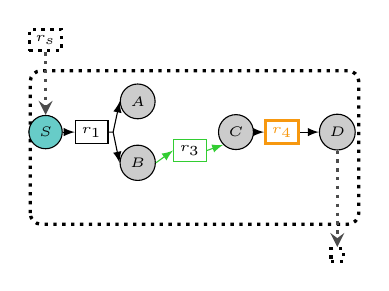
\begin{tikzpicture}[scale=0.39]\tiny
      \tikzstyle{metabolite}=[draw,circle,fill=white!80!black];
      \tikzstyle{repairmetabolite}=[draw,white!40!black, circle,fill=white!90!black,text=white!40!black,dashed];
      \tikzstyle{seed}=[draw,circle,fill=BlueGreen!70];%white!80!black
      \tikzstyle{target}=[draw,circle,fill=YellowOrange];%white!40!black
      \tikzstyle{reaction}=[draw,rectangle];
       \tikzstyle{export}=[draw,rectangle,dotted, very thick];
       \tikzstyle{exportrepair}=[draw,rectangle,dotted, very thick,white!80!black,text=white!70!black];
      \tikzstyle{repairreaction}=[draw,rectangle,white!40!black,text=white!40!black,dashed];
      \tikzstyle{solreaction}=[draw,rectangle,LimeGreen,text=black];
      \tikzstyle{initial}=[->,>=latex,thick];
      \tikzstyle{bdd}=[->,>=latex,thick];
      \tikzstyle{etiq}=[midway,fill=black!20,scale=0.5];
      \tikzstyle{stc}=[draw, rectangle, white, text=black]


      \draw [black,dotted, rounded corners, very thick] (-0.5,4) rectangle (10.2,9);
     % \node (system) [draw, rounded rectangle] at (0,0) {} (7cm,5cm);

      \node[seed] (S) at (0,7) {$S$};
      \node[metabolite] (A) at (3,8) {$A$};
      \node[metabolite] (B) at (3,6) {$B$};
      \node[metabolite] (C) at (6.2,7) {$C$};
      \node[metabolite] (D) at (9.5,7) {$D$};

      \node[reaction] (R1) at (1.5,7) {$r_{1}$};
      \node[reaction, very thick,YellowOrange] (R4) at (7.7,7) {$r_{4}$}; %LimeGreen
      %\node[solreaction] (R2) at (4.7,7.6) {$r_{2}$};
      \node[solreaction] (R3) at (4.7,6.4) {$r_{3}$};

      % R1 : S => A + B
      \draw[->,>=latex] (S.east) -- (R1.west);
      \draw[->,>=latex] (R1.east) -- (2.2,7) -- (A.west);
      \draw[->,>=latex] (2.2,7)  -- (B.west);

      % R2 : A => C
      %\draw[->,>=latex,LimeGreen] (A.east) -- (R2.west);
      %\draw[->,>=latex,LimeGreen] (R2.east) -- (C.north west);

      % R3 : B => C
      \draw[->,>=latex,LimeGreen] (B.east) -- (R3.west);
      \draw[->,>=latex,LimeGreen] (R3.east) -- (C.south west);

      % R4 : C => D
      \draw[->,>=latex] (C.east) -- (R4.west);
      \draw[->,>=latex] (R4.east) -- (D.west);

      %export G
      \node[export] (outD) at (9.5,3) {\ExportReaction};
      \draw[->,>=stealth,white!30!black,dotted, very thick] (D.south) --  (outD.north);

      %import S2
      \node[export] (inS) at (0,10) {$r_{s}$};
      \draw[->,>=stealth,white!30!black,dotted, very thick] (inS) --  (S.north);

  \end{tikzpicture}
% \end{figure}

% \end{document}
